\chapter{Αρχιτεκτονική Lambda}
Ένα από τα πιο σύνθετα προβλήματα που χρειάζεται να αντιμετωπίζουν τα Big Data συστήματα είναι η εύρεση λύσης/απάντησης σε πραγματικό χρόνο.Κατά την αρχική τους σχεδίαση, δεν υπήρχε καμία πρόβλεψη για την αντιμετώπιση αυτού του είδους των προβλημάτων και φαινόταν έξω από την σφαίρα των δυνατοτήτων τους. Με την υποστήριξη και την ανάπτυξη που έλαβαν τα χρόνια μετά την εμφάνιση τους, βοήθησαν να αναπτυχθούν και να εδραιωθούν σε όλο και περισσότερους τομείς της πληροφορικής. Ο τομέας των \textit{real-time analytics} αποδείχθηκε ένα αρκετά μεγάλο πρόβλημα, λόγω του όγκου της πληροφορίας που αποθηκεύεται σε ένα τέτοιο σύστημα. Η λύση ακόμα δεν έχει δοθεί από ένα μόνο συγκεκριμένο σύστημα αλλά έχει περιγραφτεί μια αρχιτεκτονική συστημάτων που παράγει το σωστό αποτέλεσμα, με μερικούς περιορισμούς.Η αρχιτεκτονική αυτή ονομάζεται Lambda και οι βασικές της αρχές θα αναλυθούν σε αυτό το κεφάλαιο.

\section{Επίπεδα}
Η βασική ιδέα της αρχιτεκτονικής Lambda είναι τα επίπεδα. Κάθε Big Data σύστημα που την εφαρμόζει θα αποτελεί μια σειρά από επίπεδα όπου σε κάθε επίπεδο εφαρμόζετε διαφορετικό σύστημα. Όλα μαζί τα επίπεδα λειτουργούν ως ένα ενιαίο \textit{real-time system}.Το κάθε επίπεδο έχει διαφορετικό σκοπό και ο οποίος ενεργεί σε συνδυασμό με τα αποτελέσματα των επιπέδων κάτω από αυτό.Στην πολύ απλή τους μορφή τα επίπεδα είναι αυτά που φαίνονται στο σχήμα 1.1 .

\begin{figure}[t]
\caption{Επίπεδα της Αρχιτεκτονικής Lambda}
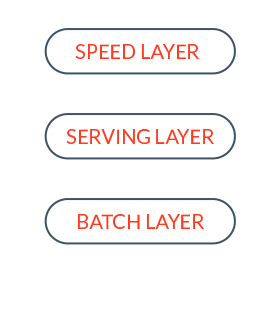
\includegraphics[width=10cm]{images/layers.png}
\centering
\end{figure}
\clearpage

\section{Query}
Αυτός ο πολύ απλός ορισμός των επιπέδων αρκεί, για αυτό το κεφάλαιο, για να γίνει κατανοητή η λειτουργία της Αρχιτεκτονικής Lambda. Όπως έχει αναφερθεί, το πρόβλημα που πρέπει να λυθεί είναι τα \textit{real-time analytics}.Αυτό μπορεί να συνοψιστεί, για λόγους απλότητας, σε μια πρόταση ως εξής:
\begin{verbatim}
query = function(all data)
\end{verbatim}

Όπου \textit{query} είναι η ερώτηση που υποβάλετε στο σύστημα, η \textit{function} είναι η συνάρτηση υπολογισμού της απάντησης πάνω στα \textit{data}, όλα τα δεδομένα που έχει αποθηκευμένα το σύστημα εκείνη την χρονική στιγμή.
\newline
Στα περισσότερα Big Data συστήματα αυτός ο υπολογισμός θα απαιτούσε από μερικές ώρες μέχρι μερικές ημέρες, δεδομένου του μεγέθους που έχουν τα δεδομένα και την πολυπλοκότητα του υπολογισμού. Για να μπορέσει να απαντηθεί ένα τέτοιο ερώτημα σε \textit{real-time} θα έπρεπε να χρησιμοποιηθούν τεράστιες υποδομές ηλεκτρονικών υπολογιστών και το κόστος, στις περισσότερες περιπτώσεις, για κάτι τέτοιο υπερβαίνει την αξία της απάντησης. Με την Αρχιτεκτονική Lambda αναμένετε η απάντηση να δοθεί σε μερικά δευτερόλεπτα έως λεπτά σε υποδομές πολύ μικρότερης κλίμακας και κόστους. 

\section{Προΰπολογισμός}
Η λύση που υλοποιεί η Αρχιτεκτονική Lambda υποστηρίζετε από τον προϋπολογισμό της απάντησης. Δηλαδή η απάντηση σε υπολογίζετε από την βασικό dataset την στιγμή που υποβάλετε η ερώτηση, αλλά έχει ήδη υπολογιστεί σε προγενέστερο χρόνο και έχει αποθηκευτεί στο σύστημα. Η προϋπολογισμένη απάντηση, στην Αρχιτεκτονική Lambda, ονομάζετε \textit{batch view}. Πλέον η προηγούμενη πρόταση έχει πάρει μια διαφορετική μορφή:
\begin{verbatim}
batch view = function (all data)
query = function (batch view)
\end{verbatim}
Τα \textit{batch view} είναι \textit{indexed} για να είναι πιο γρήγορη και εύκολη η εύρεση του σωστού \textit{batch view} και να απαντηθεί το \textit{query} μέσα στον επιθυμητό χρόνο.



\section{Batch Layer}
Το επίπεδο της Αρχιτεκτονικής που υπολογίζει τα \textit{batch view} από το \textit{dataset} ονομάζεται \textit{batch layer} και αποτελεί το πρώτο επίπεδο του συστήματος. Εκτός από τον υπολογισμό των \textit{batch view}, το \textit{batch layer} είναι υπεύθυνο για την αποθήκευση του \textit{master dataset}, δηλαδή των δεδομένων που χρησιμοποιούνται για τον υπολογισμό των \textit{batch view}. Το σύστημα που θα χρησιμοποιηθεί στο \textit{batch layer} θα πρέπει να αποθηκεύει αποδοτικά και με ασφάλεια μεγάλα μεγέθη δεδομένων που συνεχώς θα αυξάνονται, και να εφαρμόζει πάνω τους τους αλγορίθμους υπολογισμού των \textit{batch view} κατά συγκεκριμένες περιόδους. Τέτοια συστήματα ονομάζονται \textit{batch-processing
systems}. Ένα από τα πιο δημοφιλή τέτοια συστήματα είναι το \textbf{Hadoop}, το οποίο θα χρησιμοποιηθεί και σε αυτή την περίπτωση, αλλά θα περιγραφτεί αναλυτικότερα σε επόμενα κεφάλαια.
\newline
Μια απεικόνιση του \textit{batch layer} φαίνεται στο σχήμα 1.2.

\begin{figure}[t]
\caption{Batch Layer}
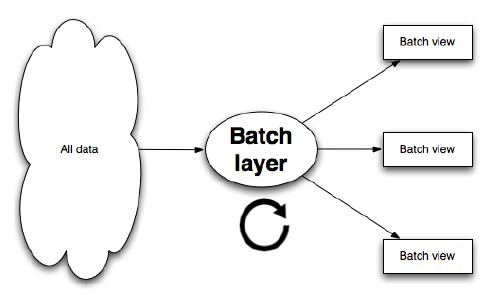
\includegraphics[width=12cm]{images/batch_layer.jpg}
\centering
\end{figure}
\clearpage

\subsection{Πλεονεκτήματα}
\begin{description}
\item[Παραλληλισμός] Το \textit{batch layer} είναι το πιο απλό και εύκολο στην χρήση επίπεδο της Αρχιτεκτονικής Lambda. Οι αλγόριθμοι που υπολογίζουν τα \textit{batch view} είναι υλοποιημένοι ως γραμμικοί αλγόριθμοι αλλά εκτελούνται παράλληλα χάρη στους μηχανισμούς που προσφέρει το \textit{batch layer}.
\item[Επεκτασιμότητα] Καθώς αυξάνετε ο όγκος των δεδομένων, θα πρέπει να αυξάνετε και το μέγεθος του συστήματος για να αντεπεξέλθει στις απαιτήσεις. Στο \textit{batch layer}, η επέκταση γίνετε απλά με την εισαγωγή νέων μηχανημάτων στο σύστημα.
\item[Ασφάλεια] Η ασφάλεια των δεδομένων που αποθηκεύονται στο \textit{batch layer} διασφαλίζετε με τους μηχανισμούς που προσφέρει το σύστημα, χωρίς να χρειαστεί να σχεδιαστούν πολύπλοκες αρχιτεκτονικές και έλεγχοι από τον διαχειριστή.
\end{description}


\subsection{Μειονεκτήματα}
Το προφανές μειονέκτημα αυτής της υλοποίησης είναι η ανάγκη το σύστημα να γνωρίζει από πριν τις ερωτήσεις που θα του υποβληθούν στο μέλλον. Δεν υπάρχει η δυνατότητα να απαντήσει, σε \textit{real-time}, ερώτηση που δεν έχει καταχωρηθεί στις γνωστές. Επίσης από την στιγμή που θα εισαχθεί μια νέα ερώτηση, υπάρχει ένα χρονικό διάστημα που χρειάζεται για τον υπολογισμό των \textit{batch view} ώστε να είναι σε θέση να την απαντήσει. Αυτό το μειονέκτημα καθιστά την Αρχιτεκτονική Lambda λύση για ένα υποσύνολο των προβλημάτων που ανάγονται σε \textit{real-time analytics} προβλήματα.